\chapter{CONCLUSIONS AND FUTURE WORK}
\thispagestyle{plain}

\label{Conclusions}

% Summarize the work
   % Explained how to define system-level properties
   % Outlined the framework for learning a forward mapping
   % Outlined the framework and provided an algorithm for learning the reverse mapping
   % Demonstrated with emperical results that my approach is accurate and efficient.

% The research project reached its aims
   % what did I try to achieve?
      % The main goal of the \framework is to bridge the gap between agent-level parameters and system-level properties.

      %\item Domain independent: The design of \fw should minimize the amount of configuration that is needed for each new domain;
      %\item Algorithm independent: any regression algorithm should be able to be applied with \fw;
      %\item Accurate: \fw should generate accurate predictions and control suggestions; and
      %\item Fast for the user -- interactions with the models generated by \fw should require minimal computational time.

   % How did I achieve those goals?
      % Generating meta-models of the agent-based models
      % Previous approaches only returned one point, which gives a possible configuration, but not \fw!





\section{Future Work}

In the course of the research presented in this dissertation, a number of possible directions for future work have arisen.
Each of the following subsections discuss a possible subproblem in ABM meta-modeling or extensions to \fw that could produce interesting results.

\section{Extension: Specifying Ranges for System-level Properties}
\label{sec:ranges}

One of the major problems with SCI is that queries can easily become overspecified.
In the case of overspecification, the reverse mapping will not return any solutions, since they do not exist.
To avoid this problem, SCI can be altered process ranges of system-level property values, instead of specific values.
This provides some leeway and allows for more possibility of intersections.
Instead of the solution of the reverse-mapping query being a hyperplane, it is now a hyperspace.
The query plane used to intersect with the reverse mapping is also now a hyperspace bounded by two hyperplanes.

This extension complicates the implementation significantly.
In order to implement this in SCI, the equations used would now be inequalities.
Any point that is satisfied by the set of inequalities over all simplexes could satisfy the system-level property ranges.
The implementation of this approach is left as future work.

The Quad-Tree (QT) approach for inverting the forward mapping is intended to be a simpler to implement approach than SCI.
Also, specifying ranges for system-level properties is more natural in QT than in SCI.
QT performs the same tasks as SCI, but instead returns a set of subspaces that must or could possibly contain configurations that satisfy the desired system-level property configuration.
In general, a quad-tree is a tree data structure in which each node either has zero or four children.
They can be used to iteratively segregate a two-dimensional space into several subspaces in order to give certain portions of the space more detail.
Quad-trees use a notion of ``black", ``gray", and ``white" cells: black cells represent a subspace in which all values are black, white cells represent a subspace in which all values are white, and gray cells represent a subspace in which some values are white sand some values are black.
The benefit of using a quad-tree structure is black and white cells do not need to be expanded, as all their values are already determined.
However, gray cells are broken down further by segregating its space into four children, which may be black, gray, or white.
Grey cells can be broken down as many times as desired, but in general is capped at a certain depth, which I call the ``granularity depth."

The idea of quad-trees are used in the reverse mapping to approximate the solution space.
Black nodes are ones in which all values within the subspace match the query,
white nodes are ones in which none of the values within the subspace match the query,
and gray nodes are ones in which some of the values within the subspace match the query.
Instead of using squares to split the subspaces, QT must use hypercubes, as the configuration space is typically not two-dimensional.
QT returns all the gray cells and black cells found by this approach as an answer to a user's query.

Gray nodes are broken down iteratively until the granularity depth is reached.
QT breaks down a hypercube (a pair of simplexes) by querying the forward mapping for the points needed to break a single $n$-dimensional hypercube into $2^n$ hypercubes (e.g., split a line into two lines, a square into four squares, a cube into eight cubes, etc.).
Each new hypercube is then evaluated to see whether it contains the desired system-level property values or not, which can be determined by comparing the desired system-level property with the observed maximum and minimum among the corners of each hypercube.
If the desired system-level property value is less than the maximum, and greater than the minimum, then possibly an intersection satisfying all system-level properties exists within this hypercube.
If one of the values is not contained within this range, then the hypercube is marked as ``white" and does not need to be expanded further.

This approach has the benefit that the intersections of hyperplanes do not need to be calculated, which may be difficult to implement.
Although it is less accurate and the space it returns is not continuous, it serves the purpose of the reverse mapping in many ways.
It still returns configurations that the user should use to generate the behavior and can still be visualized to show the nature of the configurations that generate a particular system-level property.

Another motivation for using QT over SCI is in specifying ranges for system-level properties is difficult to represent in SCI because all the equations are inequalities.
Meanwhile, the implementation in QT is quite simple because either hypercubes contain the values, or do not.
Details on the uses of ranges in querying the reverse mapping are discussed in Section \ref{sec:ranges}.

\begin{figure}[ht]
\centering
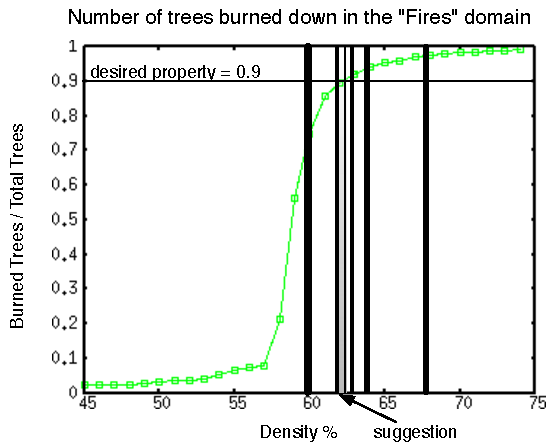
\includegraphics[scale=1]{images/QTfires.pdf}
\caption{The subspaces generated by QT represent a range of configurations that are close to satisfying the desired system-level property.}
\label{fig:qtfires}
\end{figure}

The usage of QT on the fires domain is visualized in Figure \ref{fig:qtfires}.
The thicker bars represent earlier separation.
First, the space was split into the ranges 45--60 and 60--75.
The system-level property ranges from .02 to .7 in the 45--60 subspace, so this space can be ignored in future divisions because it does not contain the value .9.
The other half is subdivided at 67.5.
This process continues five times, which is the granularity depth in this case.
In a situation in which several solutions are possible, several subspaces will be returned as candidate configuration spaces.


\begin{figure}[ht]
\centering
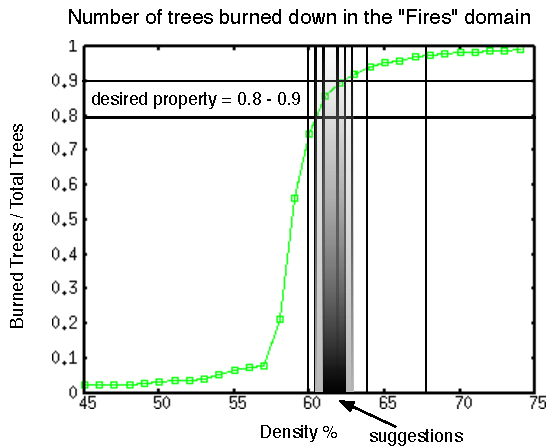
\includegraphics[scale=1]{images/QTfiresranges.pdf}
\caption{The subspaces generated by QT represent a range of configurations that are close to satisfying ranges of the desired system-level property.}
\label{fig:qtfiresranges}
\end{figure}
To handle ranges of system-level property values, only minor modifications to QT must be done.
The space is subdivided in the same way as standard QT, however, spaces that lie entirely within the ranged are marked as ``black" and do not need to be subdivided further.
Ranges marked as ``white" do not need to be subdivided either.
Gray areas are inspected more closely in order to increase the detail of the reverse mapping solution.
A set of configuration spaces are returned that represent the configurations that will satisfy the system-level property range.
This process is visualized in Figure \ref{fig:qtfiresranges}.



The caveat with this approach is in non-monotonically changing domains, the maximum and minimum values at the corners do not necessary accurately describe the maximum and minimum within the hypercube.
If there exists a local minima or local maxima within a cube, the feature will be ignored.
To avoid this problem, the starting grid of hypercubes should be sufficiently detailed.



\subsection{Adaptive Meta-models}

In some agent-based models a hidden property may continue to change.
A hidden property is a feature of the environment that changes the behavior of the agents in some way, but is not directly detectable.
In the case that the hidden property does not change, the learned mappings will adapt to this hidden variable and the mappings will continue to be accurate.
However, in cases in which the hidden property changes over time, the learned mappings must be adaptive, as the value of the hidden property is not part of the configuration vector.
Because of a changing hidden property, the system-level behavior of a system can change over time, yet be still running the same configuration.

Wind in a flocking ABM serves as a good example of this phenomena.
A strong wind can change the behavior of a flocking system to be less cohesive.
However, the value of the wind is not predictable, which can cause predictions about the system to be erroneous.

To tackle this problem, the meta-models built by the forward and reverse mapping must be adaptive to the current conditions in the ABM.
I propose that an online optimization technique that incrementally adjusts the behavior of the system to compensate for hidden changes in the system.
A continuous stream of current system-level property values will be going into the system.
The forward mapping will predict what should be happening with this configuration and is compared to the actual system-level behavior.
The distance between the predicted and actual is minimized by incrementally changing the configuration in order to minimize this gap.
Over time, the difference between the predicted and actual value will converge.

This is an optimization approach, but is different from standard optimization because the initial starting position provided by the forward mapping is presumably close to the optimal configuration.
Also, the derivative of the mapping can be used in a gradient ascent approach, with the gradient already known.
Hidden variables typically will not change the nature of the system, only the specific values.
That is, increasing one configuration parameter is likely to have the same sort of effect, but not exactly.


% hidden properties that can change

\subsection{Correlated System-level Properties}
% need to predict all system-level properties as one.

One of the major assumptions used for the \fw approach to learning the reverse mapping is that the system-level properties are not correlated.
This allows us to split the reverse mapping problem into a number of reverse mapping subproblems (one per system-level property).
However, if the properties are correlated, the result of the reverse mapping may be inaccurate.

For example, consider two system-level properties $a$ and $b$ are correlated such that $a \cdot b^2 = 1$.
Presume that \fw, while solving the reverse-mapping problem, averages $a$ and $b$ separately for the following two instances: $a=100, b=\frac{1}{10}$ and $a=400, b=\frac{1}{20}$.
The averages are $a=250, b=\frac{1}{15}$, however, $250 \cdot \frac{1}{15} \neq 1$, which clearly is not a valid instance.

To avoid this problem, a multi-variate learning approach must be taken.
The forward mapping must be learned with a multi-variate regression algorithm, which must then be inverted in a multi-variate manner, as well.
This type of approach will consider all properties at once.





\subsection{The Reverse-mapping Approach as a General Algorithm}

% the SCI approach and the quad-tree method
